% Last Update: $Id: sshd_main.tex 53967 2018-09-26 16:22:35Z kristov $
\section {SSHD - Secure Shell, Secure Copy}

Eine Secure-Shell bietet die Möglichkeit, eine verschlüsselte Verbindung mit
dem fli4l-Router aufzunehmen. Außerdem können mit dem Secure-Copy-Befehl
Dateien verschlüsselt auf den fli4l-Router übertragen werden. Wird zusätzlich
eine \jump{SSHDPUBLICKEYN}{Public Key Anmeldung} benutzt, können Befehle auf
dem fli4l-Router und Dateiübertragungen auch scriptgesteuert ausgeführt
werden. Ab der Version 2.1.7 gibt es nur noch einen SSH2 Server.

\subsection {Installation des Secure-Shell-Dienstes}

\begin{description}

\config {OPT\_SSHD}{OPT\_SSHD}{OPTSSHD}

  Standard-Einstellung: \var{OPT\_\-SSHD='no'}

  Soll der Zugriff auf den Router mittels ssh ermöglicht werden, bedarf es
  der Änderung auf von \var{OPT\_\-SSHD} auf \var{'yes'}. Dies installiert den
  ssh-Server Dropbear auf dem fli4l-Router. Dies ermöglicht auch das Kopieren
  von Dateien auf den Router.

\config {SSHD\_ALLOWPASSWORDLOGIN}{SSHD\_ALLOWPASSWORDLOGIN}{SSHDALLOWPASSWORDLOGIN}

  Standard-Einstellung: \var{SSHD\_ALLOWPASSWORDLOGIN='yes'}

  Wird \var{SSHD\_ALLOWPASSWORDLOGIN} auf \var{'no'} eingestellt, ist die
  Anmeldung mit ssh über ein Passwort auf dem fli4l-Router nicht mehr
  möglich. Die Anmeldung kann dann nur noch mittels privatem/öffentlichem
  Schlüsselpaar (private/public key) erfolgen. Dies setzt voraus, dass ein
  \jump{SSHDPUBLICKEYN}{öffentlicher Schlüssel} auf dem Router hinterlegt ist.

\config {SSHD\_CREATEHOSTKEYS}{SSHD\_CREATEHOSTKEYS}{SSHDCREATEHOSTKEYS}

  Standard-Einstellung: \var{SSHD\_CREATEHOSTKEYS='no'}

  Ein ssh-Server benötigt einen sogenannten Hostkey, der weltweit
  einmalig sein sollte, damit sich der ssh-Server eindeutig gegenüber
  einem ssh-Client identifizieren kann. Das sshd opt-Paket liefert
  zwar einen Hostkey mit, um das erste Einloggen auf dem fli4l-Router
  per ssh-Client zu erlauben, aber der mitgelieferte Hostkey sollte so
  schnell wie möglich durch einen selbst generierten, nur Ihnen bekannten
  Hostkey ersetzt werden.
  Die Generierung eines eigenen Hostkeys ist deshalb so wichtig, weil
  nur auf diese Weise Schutz gegen so genannte Man-in-the-Middle-Attacken
  möglich ist. Ihr ssh-Client bemerkt es, wenn ein Cracker vorgibt, Ihr
  fli4l-Router zu sein, da dem Cracker dessen Hostkey nicht bekannt ist. Ihr
  ssh-Client warnt Sie daraufhin mit einer Meldung, dass der Hostkey sich
  geändert hat.

  Die Erzeugung Ihres eigenen Hostkeys geschieht vollkommen automatisch, sobald
  Sie die Einstellung \var{SSHD\_CREATEHOSTKEYS} auf \var{'yes'} setzen. Dieser
  Vorgang ist sehr rechenintensiv und kann deshalb die Bootzeit um mehrere
  Minuten verlängern.  Wenn der fli4l-Router mit aktiviertem
  \var{SSHD\_CREATEHOSTKEYS} Eintrag startet, wird ein (oder mehrere)
  Hostkey(s) in dem Verzeichnis \var{/tmp/ssh} erzeugt.  Die Dateien die dort
  stehen, kopieren Sie in das Verzeichnis \var{etc/ssh} unterhalb Ihres config
  Verzeichnisses (auf dem Rechner, auf dem sie fli4ls Bootmedium erzeugen). 
  In meinem Fall sieht ein Directorylisting des config.babel
  Verzeichnisses so aus:

  \begin{figure}[htbp]
    \centering
    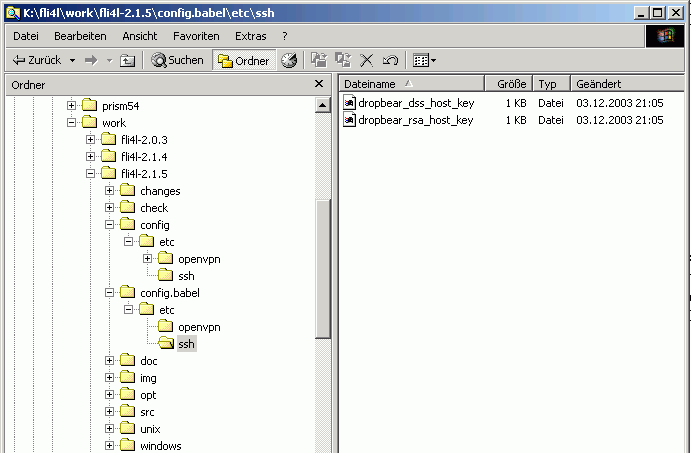
\includegraphics[width=\columnwidth]{etc_ssh_dir}
    \caption{Verzeichnisstruktur fli4l}
    \label{fig:etc_ssh_dir}
  \end{figure}

  Beachten Sie, dass unterhalb des \var{config} Verzeichnis 
  erst das Verzeichnis etc kommt und darunter dann das Verzeichnis ssh. Und
  genau dorthin muss der oder die eben erzeugte(n) Hostkey(s) kopiert
  werden. Ab der fli4l Version 2.1.5 werden Dateien die unterhalb
  Ihres config Verzeichnisses stehen vorrangig vor den Dateien aus dem
  opt Verzeichnis behandelt. Dadurch werden bei dem nächsten Update
  Ihres fli4l-Routers die Dateien aus dem Verzeichnis \var{config/etc/ssh}
  eingebunden und nicht die Dateien, die im Verzeichnis \var{opt/etc/ssh}
  stehen. So ist es möglich für jeden fli4l-Router, den Sie
  konfigurieren, einen eigenen Hostkey zu benutzen. Wenn Sie die
  fli4l-Routerdateien erzeugen, erscheint ziemlich zum Schluss die
  Meldung \glqq{}appending config specific files to opt.img ...\grqq{}.
  Dort werden dann alle Dateien aufgelistet, die aus Ihrem
  config Verzeichnis kommen und nicht aus dem opt Verzeichnis.

\begin{verbatim}
#
# appending config specific files to opt.img ...
#
etc/ssh/dropbear_dss_host_key
etc/ssh/dropbear_rsa_host_key
\end{verbatim}

  Wenn Sie einen neuen Hostkey erzeugt haben, setzen Sie danach den
  Wert \var{SSHD\_\-CREATEHOSTKEYS} wieder auf \var{'no'}, damit die
  Startskripte des fli4l-Routers nicht ständig einen neuen Hostkey generieren.

  Wenn Sie sich nach dem Update des Hostkey auf Ihrem fli4l-Router
  anmelden, wird eine (je nach Programm unterschiedliche) Warnmeldung
  von Ihrem ssh-Client ausgegeben, die Sie auf einen geänderten Hostkey
  hinweist. Das ist normal, da Sie ja gerade den von fli4l mitgelieferten
  Hostkey gegen den von Ihnen erzeugten Hostkey ausgetauscht haben.
  Befolgen Sie die Hinweise Ihres ssh-Client, wie Sie den geänderten
  Hostkey permanent übernehmen können. Sollten Sie diese Warnmeldung zu
  einem späteren Zeitpunkt noch einmal bekommen, sollten Sie in jedem Fall
  prüfen, warum diese Warnung ausgegeben wurde und nicht einfach blind den
  geänderten Hostkey akzeptieren.

\begin{verbatim}
@@@@@@@@@@@@@@@@@@@@@@@@@@@@@@@@@@@@@@@@@@@@@@@@@@@@@@@@@@@
@    WARNING: REMOTE HOST IDENTIFICATION HAS CHANGED!     @
@@@@@@@@@@@@@@@@@@@@@@@@@@@@@@@@@@@@@@@@@@@@@@@@@@@@@@@@@@@
IT IS POSSIBLE THAT SOMEONE IS DOING SOMETHING NASTY!
Someone could be eavesdropping on you right now (man-in-the-middle attack)!
It is also possible that the RSA host key has just been changed.
The fingerprint for the RSA key sent by the remote host is
ca:a4:ab:e7:af:d8:68:05:d3:1f:e6:15:08:d6:ed:36.
Please contact your system administrator.
Add correct host key in /home/babel/.ssh/known_hosts to get rid of this message.
Offending key in /home/babel/.ssh/known_hosts:7
Password authentication is disabled to avoid man-in-the-middle attacks.
\end{verbatim}

\config {SSHD\_PORT}{SSHD\_PORT}{SSHDPORT}

  Standard-Einstellung: \var{SSHD\_PORT='22'}

  Mit \var{SSHD\_PORT} kann abweichend vom Standard ein Port
  angegeben werden, auf dem der ssh-Server laufen soll.

  Möchte man den ssh-Zugang auch von außen erlauben, ist
  \jump{PFNEWCONFIG}{\var{INPUT\_ACCEPT\_PORT\_x}} anzupassen.

  Die Befehle, um von einem Unix-/Linux-Rechner über das SSH-Protokoll
  auf fli4l zuzugreifen, lauten:
  \begin{itemize}
  \item ssh - Secure Shell
  \item scp - Secure Copy
  \end{itemize}

  Entsprechende Programme für Windows sind ebenso verfügbar, s.
  auch:
  \linebreak
  \altlink{http://www.chiark.greenend.org.uk/~sgtatham/putty/}
  \linebreak
  \altlink{http://winscp.net/eng/docs/lang:de}
  \linebreak
  \altlink{http://www.tectia.com/de/de.iw3}

\config {SSHD\_PUBLIC\_KEY\_N}{SSHD\_PUBLIC\_KEY\_N}{SSHDPUBLICKEYN}

  Standard-Einstellung: \var{SSHD\_PUBLIC\_KEY\_N='0'}

  \var{SSHD\_PUBLIC\_KEY\_N} beschreibt die Anzahl der
  öffentlichen Schlüssel, die auf den fli4l-Router kopiert werden
  sollen.

  SSH gestattet die Authentifizierung mit Hilfe von asymmetrischen
  Verschlüsselungsverfahren. Dabei erfolgt die Authentifizierung
  anstatt über Nutzername und Passwort über Nutzername und einem
  Public-/Privatekey.  Damit kann man sich die Eingabe eines
  Passwortes sparen.  Das Schlüsselpaar erzeugt man mit Hilfe von
  ssh-keygen (oder puttygen, wenn putty unter Windows als ssh-Client
  eingesetzt wird). Optional kann beim Schlüsselerzeugen eine
  Passphrase (also ein Passwort, das man braucht, wenn man
  den Schlüssel benutzen will) vergeben werden, welche die Sicherheit noch
  zusätzlich erhöht. Benutzt man Passphrases sollte man über den
  Einsatz eines Schlüsselagenten nachdenken (siehe ssh-agent oder
  pageant).

  \wichtig{Der private Teil des Schlüsselpaares,
  ist so sorgfältig zu behandeln wie ein Passwort, da er die gleiche
  Funktion erfüllt. Der private Teil des Schlüssel wird bei dem
  ssh-Client hinterlegt. Der öffentliche Teil des Schlüssel wird für
  den fli4l-Router gebraucht und mit \var{SSHD\_PUBLIC\_KEY\_x} oder
  \var{SSHD\_PUBLIC\_KEYFILE\_x} zur Verfügung gestellt.}

  Für weitere Informationen siehe die manual Pages von ssh und
  Konsorten bzw. die Dokumentation zu putty
  (\altlink{http://www.chiark.greenend.org.uk/~sgtatham/putty/}).

\config {SSHD\_PUBLIC\_KEY\_x}{SSHD\_PUBLIC\_KEY\_x}{SSHDPUBLICKEYx}

  Für jeden Nutzer, der über ssh Zugang zum fli4l-Router erlangen möchte,
  kann hier der öffentliche Teil des Schlüssel angegeben werden.  Am
  einfachsten geht das per Cut-and-Paste aus einem Terminalfenster
  heraus. Das könnte z.B. in etwa wie folgt aussehen:

\begin{example}
\begin{verbatim}
        SSHD_PUBLIC_KEY_1='1024 ... nutzername@hostname'
\end{verbatim}
\end{example}

 \wichtig{Der Schlüssel enthält keine Zeilenumbrüche. Bei Cut-and-Paste
 aus puttygen heraus werden aber eventuell selbige eingefügt. Diese
 Zeilenumbrüche müssen wieder entfernt werden.}

  Zur Zeit werden Schlüssel für die folgenden Verschlüsselungsverfahren
  unterstützt:
  \begin{itemize}
  \item DSA
  \item RSA
  \item ECDSA
  \end{itemize}

\config {SSHD\_PUBLIC\_KEYFILE\_N}{SSHD\_PUBLIC\_KEYFILE\_N}{SSHDPUBLICKEYFILEN}

  Standard-Einstellung: \var{SSHD\_PUBLIC\_KEYFILE\_N='0'}

  Anstatt den Inhalt des öffentlichen Teil des Schlüssel in die
  sshd.txt Datei zu kopieren, können Sie den öffentlichen Teil des
  Schlüssel auch direkt in das opt-Archiv kopieren lassen. Das
  funktioniert genauso wie bei \var{SSH\_CREATEHOSTKEYS} beschrieben
  wurde. Kopieren Sie Ihren öffentlichen Teil des Schlüssel in das
  Verzeichnis \var{$<$config$>$/etc/ssh}.

\config {SSHD\_PUBLIC\_KEYFILE\_x}{SSHD\_PUBLIC\_KEYFILE\_x}{SSHDPUBLICKEYFILEx}

  Der Dateiname des öffentlichen Teil des Schlüssels im
  \var{$<$config$>$/etc/ssh} Verzeichnis.

\begin{example}
\begin{verbatim}
        SSHD_PUBLIC_KEYFILE_1='root@fli4l'
\end{verbatim}
\end{example}

  Zur Zeit werden Schlüssel für die folgenden Verschlüsselungsverfahren
  unterstützt:
  \begin{itemize}
  \item DSA
  \item RSA
  \item ECDSA
  \end{itemize}

\config {SSH\_CLIENT\_PRIVATE\_KEYFILE\_N}{SSH\_CLIENT\_PRIVATE\_KEYFILE\_N}{SSHCLIENTPRIVATEKEYFILEN}

  Standard-Einstellung: \var{SSH\_CLIENT\_PRIVATE\_KEYFILE\_N='0'}

  Wenn Sie mit dem ssh oder plink Client private Schlüssel zur
  Anmeldung an einen ssh Server benutzen wollen können Sie diese in
  das Verzeichnis \var{$<$config$>$/etc/ssh} kopieren. Das funktioniert genauso
  wie bei \var{SSH\_CREATEHOSTKEYS} beschrieben wurde. Kopieren Sie
  Ihren privaten Teil des Schlüssel in das Verzeichnis
  \var{$<$config$>$/etc/ssh}. Private Schlüssel im OpenSSH-Format
  werden automatisch bei jedem Startvorgang von fli4l ins das dropbear-Format
  konvertiert.
  
\config {SSH\_CLIENT\_PRIVATE\_KEYFILE\_x}{SSH\_CLIENT\_PRIVATE\_KEYFILE\_x}{SSHCLIENTPRIVATEKEYFILEx}

  Der Dateiname des privaten Teil des Schlüssels im
  \var{$<$config$>$/etc/ssh} Verzeichnis.

\begin{example}
\begin{verbatim}
        SSHD_PRIVATE_KEYFILE_1='babel@rootserver'
\end{verbatim}
\end{example}

  Zur Zeit werden Schlüssel für die folgenden Verschlüsselungsverfahren
  unterstützt:
  \begin{itemize}
  \item DSA
  \item RSA
  \item ECDSA
  \end{itemize}

\end{description}

\subsection {Installation des dbclients}

\begin{description}

\config {OPT\_SSH\_CLIENT}{OPT\_SSH\_CLIENT}{OPTSSHCLIENT}

  Standard-Einstellung: \var{OPT\_SSH\_CLIENT='no'}

  Wenn man einen reinen ssh2/scp Client benutzen möchte, kann man den
  dbclient von dropbear durch Setzen von \var{OPT\_SSH\_CLIENT='yes'}
  aktivieren. Dieser Client hat den Vorteil, dass er sich viel
  Programmcode mit dem dropbear ssh Server teilt. Dadurch wird sehr
  viel Platz im OPT--Archiv gespart. Der dbclient ist weitgehend
  kompatibel mit dem ssh/scp Client, die Befehlsparameter sind ähnlich. Es
  wird auch ein symbolischer Link auf /usr/bin/ssh bzw. /usr/bin/scp angelegt,
  damit ein gewohntes ssh $<$host$>$ bzw. scp $<$source$>$ $<$target$>$ funktioniert.

  Wenn man die dbclient bekannten Hostkeys permanent speichern will muss
  man die Datei known\_hosts auf dem Verzeichnis /.ssh auf dem
  fli4l--Router in das config/etc/ssh kopieren. Das geschieht
  ähnlich wie mit einem erzeugten Hostkey. In dem folgenden Beispiel
  ist das ausgepackte fli4l Verzeichnis (in der die fli4l-Bootmedium
  erzeugt wird) in /home/babel/fli4l-\version~zu finden. Die
  Konfigurationsdateien liegen alle im Verzeichnis config.babel.

\begin{example}
\begin{verse}
\texttt{cd /home/babel/fli4l-\version}\\
\texttt{mkdir -p config.babel/etc/ssh}\\
\texttt{scp fli4l:/.ssh/* config.babel/etc/ssh}
\end{verse}
\end{example}

\end{description}

\subsection {Installation des plink Clients}

\begin{description}

\config {OPT\_PLINK\_CLIENT}{OPT\_PLINK\_CLIENT}{OPTPLINKCLIENT}

  Standard-Einstellung: \var{OPT\_PLINK\_CLIENT='no'}

  Installiert auf dem fli4l-Router einen ssh1/ssh2/telnet Client. Das
  plink Programm ist die Unixversion des bekannten PuTTY Programms für
  Windows. Ein Aufruf von plink auf dem fli4l-Router gibt eine
  Hilfeseite für die Benutzung von plink aus.

  Wenn man die plink bekannten Hostkeys permanent speichern will muss
  man die Datei sshhostkeys auf dem Verzeichnis /.putty auf dem
  fli4l--Router in das config/etc/plink kopieren. Das geschieht
  ähnlich wie mit einem erzeugten Hostkey. In dem folgenden Beispiel
  ist das ausgepackte fli4l Verzeichnis (in der das fli4l-Bootmedium 
  erzeugt wird) in /home/babel/fli4l-\version~zu finden. Die
  Konfigurationsdateien liegen alle im Verzeichnis config.babel.

\begin{example}
\begin{verse}
\texttt{cd /home/babel/fli4l-\version}\\
\texttt{mkdir -p config.babel/etc/plink}\\
\texttt{scp fli4l:/.putty/* config.babel/etc/plink}
\end{verse}
\end{example}

\end{description}

\subsection {Installation des sftp-server}

\begin{description}

\config {OPT\_SFTPSERVER}{OPT\_SFTPSERVER}{OPTSFTPSERVER}

  Standard-Einstellung: \var{OPT\_SFTPSERVER='no'}

  Installiert auf dem fli4l-Router einen sftp-server. 

\end{description}

\subsection{Literatur}
Dropbear SSH2 Site: \altlink{http://matt.ucc.asn.au/dropbear/dropbear.html}

Erste Version der Dokumentation von
Claas Hilbrecht $<$babel@fli4l.de$>$, im April 2004
